\def\hs#1{\hspace*{#1ex}}
\def\mycup{\, \cup \,}
\def\mycap{\, \cap \,}
\def\sc{.9cm}
\def\fillc{orange!60!white}
\def\downsh{-2.7}
\def\rightsh{3.3}
\def\recwd{3}
\def\leftcirc{(1.2,1) circle (.6)}
\def\rightcirc{(1.8,1) circle (.6)}
\def\midpt{(1.5,0)}
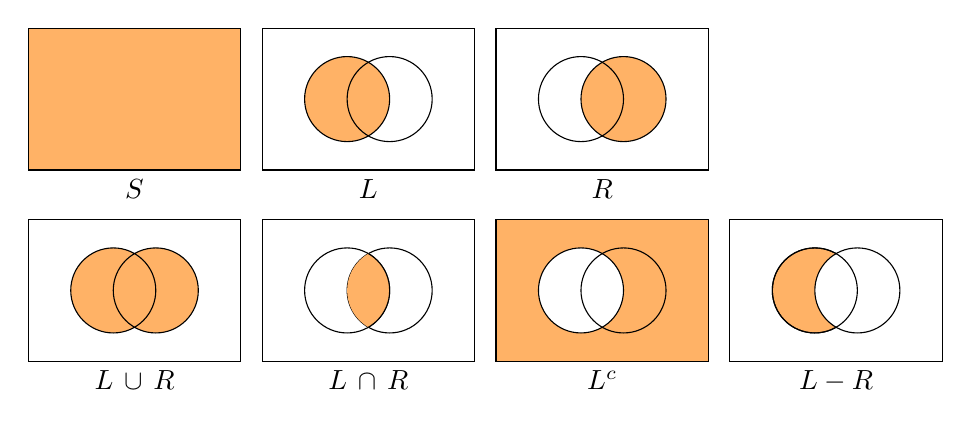
\begin{tikzpicture} [x=\sc, y=\sc]
\draw [fill=\fillc] (0,0) rectangle (\recwd,2);
\node at \midpt [below] {$S$};
\begin{scope} [shift={(\rightsh,0)}]
  \draw (0,0) rectangle (\recwd,2);
  \draw [fill=\fillc] \leftcirc;
  \draw \rightcirc;
  \node at \midpt [below] {$L$};
\end{scope}
\begin{scope} [shift={(2*\rightsh,0)}]
  \draw (0,0) rectangle (\recwd,2);
  \draw [fill=\fillc] \rightcirc;
  \draw \leftcirc;
  \node at \midpt [below] {$R$};
\end{scope}
\begin{scope} [shift={(0,\downsh)}]
  \draw (0,0) rectangle (\recwd,2);
  \draw [fill=\fillc] \leftcirc \rightcirc;
  \node at \midpt [below] {$L\mycup R$};
\end{scope}
\begin{scope} [shift={(\rightsh,\downsh)}]
  \draw (0,0) rectangle (\recwd,2);
  \draw \leftcirc;
  \begin{scope}
    \draw [clip] \rightcirc;
    \draw [fill=\fillc] \leftcirc;
  \end{scope}
  \node at \midpt [below] {$L\mycap R$};
\end{scope}
\begin{scope} [shift={(2*\rightsh,\downsh)}]
  \draw [fill=\fillc] (0,0) rectangle (\recwd,2);
  \draw [fill=white] \leftcirc;
  \draw \rightcirc;
  \node at \midpt [below] {$L^c$};
\end{scope}
\begin{scope} [shift={(3*\rightsh,1*\downsh)}]
  \draw (0,0) rectangle (\recwd,2);
  \draw [fill=\fillc] \leftcirc;
  \draw [fill=white] \rightcirc;
  \draw \leftcirc;
  \node at \midpt [below] {$L-R$};
\end{scope}
\end{tikzpicture}

